\documentclass[a4paper, 12pt]{report}
\usepackage{monapack}
\usepackage{siunitx}
\usepackage{caption}
\usepackage{graphicx}
\usepackage{subcaption}
\usepackage{hyperref}
\usepackage[bottom]{footmisc}
\captionsetup[table]{skip=5pt}

%Proměnné
\student{Milan Jiříček}
\trida{B4.I}
\obor{18-20-M/01 Informační technologie}
\bydliste{Čenkov u Bechyně 3, 391 65 Bechyně}
\datumNarozeni{10. 11. 2001}
\vedouci{Ing. Břetislav Bakala}
\nazevPrace{Dálkové ovládání zásuvek NETIO}
\cisloPrace{12}
\skolniRok{2020/2021}
\reditel{Ing. Jiří Uhlík}

%Zadání
\begin{document}

	\titulniStrana
	\anotace
		Maturitní práce se zaměřuje na porovnání platforem ESP8266 a ESP32. Cílem je vytvořit ovladač pro ovládání zásuvek značky NETIO s webovou aplikací pro konfiguraci a zjistit, která platforma je vhodná pro realizaci funkčního vzorku z hlediska spotřeby energie a~reakční doby.
	\annotation
		The graduation thesis focuses on the comparison of the ESP8266 and ESP32 platforms. The goal is to create a driver for controlling NETIO sockets with a web application for configuration and to find out which platform is suitable for the implementation of a~functional sample in terms of energy consumption and response time.
	\podekovani
		Chtěl bych poděkovat panu učiteli Ing.~Břetislavovi Bakalovi za odborné vedení práce a~cenné rady, které mi pomohly tuto práci zkompletovat. Rád bych také poděkoval  technickému řediteli Ing.~Břetislavovi Bakalovi ml. společnosti NETIO products a.s. za cenné rady, věcné připomínky a~vstřícnost při konzultacích a~vypracování bakalářské práce. V~neposlední řadě chci poděkovat Mgr. Haně Maříkové a~Mgr.~Vladimíře Špirhanzlové za~pomoc při gramatické a~stylistické kontrole.
	\tableofcontents

	\chapter{Úvod}
	%Teorie
	\chapter{Teoretický úvod do problematiky}

		\section{Zásuvka NETIO}

		\section{Platforma ESP}
			ESP jsou rodina mikročipů od společnosti \textbf{Espressif Systems}.
			\subsection{ESP8266}

				\subsubsection{Historie}
					ESP8266 je levný mikročip, který umí využívat WiFi. První chip, který se dostal na světlo světa byl v modulu \textbf{ESP-01}. Tento modul dokázal připojit se na WiFi síť a provádět jednoduché TCP/IP spojení. Získal si velkou oblibu díky nízké ceně. Jsou vhodné pro IoT jako například automatizace, zabezpečení, chytré domy atd.
				\subsubsection{Specifikace}
					Pro tuto maturitní práci bude použit modul \textbf{WT8266-S1}, který je vytvořen společností \textbf{Wireless-Tag}. Je založen na mikročipu ESP8266.\\
					ESP8266 integruje vylepšenou verzi procesoru \textbf{L106 Diamond series 32-bit} vytvořený firmou \textbf{Tensilica} s podporou frekvencí 80 \si{MHz} a 160 \si{MHz} a RTOS\footnote{Operační systém v realném čase}.
					K dispozici je 36 \si{KB} RAM a 16 \si{Mbit} Flash paměti. Intergrovaný v systému je také 10 bitový analog-digitální převodník. Modul podporuje standard {\bf IEEE802.11 b/g/n}	\footnote{Standard pro lokální bezdrátové sítě} a sadu protokolů TCP/IP. WiFi 2,4 \si{GHz} umožňuje WPA/WPA2 \footnote{Chráněný přístup k WiFi}, rychlost až 72,2 \si{Mbps} a ke komunikaci využívá anténu PCB. Zařízení má 16 GPIO pinů\footnote{Vstupně výstupní pin} (\viz{ESP8266_piny}). Také obsahuje:
					\begin{itemize}
						\item {\bf UART} - univerzální asynchronní přijímač-vysílač pro sériový přenos
						\item {\bf I$^2$C} - seriová sběrnice o dvou vodičích pro nízkorychlostní zařízení
						\item {\bf I$^2$S} - seriová sběrnice pro digitální audio
						\item {\bf SPI} - seriové periferní rozhraní pro komunikaci mezi mikroprocesorem a integrovanými obvody
						\item {\bf rozhraní HSPI} - externí SPI pro připojení displeje či externí Flash
						\item {\bf PWM rozhraní} - 4 kanálová pulzně šířková modulace pro přenos analogového signálu pomocí dvouhodnotného signálu
					\end{itemize}

					\begin{figure}[h]
						\centering
						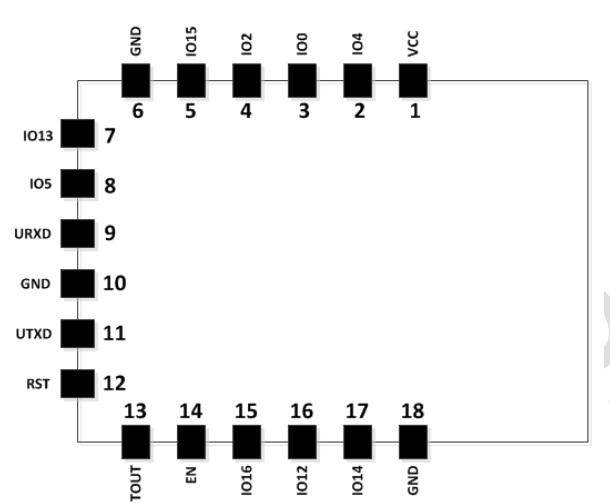
\includegraphics[width=9cm]{ESP8266_piny.png}
						\caption{ESP8266 pinout}
						\label{ESP8266_piny}
					\end{figure}

					\subsubsection{Deep sleep} \label{subsub:Deep sleep}
						Platforma ESP lze také uvést do úsporného režimu. Jednoduše to znamená vypnutí nedůležitých částí pro ustálený stav. ESP8266 celkově nabízí 3 druhy úsporných režimů. Modem, light a deep. Pro moji maturitní práci použiji deep sleep, který je nejúspornějších. Kromě {\bf RTC}\footnote{Hodiny realného času} se vše vypne, včetně CPU či WiFi. V tomto režimu je také možné uchovat data v tzv. RTC paměti, která jsou dostupná i po obnovení. Průměrná spotřeba je 20 \si{\micro A} a je vhodný pro jakýkoliv projekt na akumulátor či baterii. \\
						Probuzení ESP probíhá, buď po nastaveném čase, kde je nutné připojit pin {\bf GPIO 16} tzv. wake-up pin na {\bf RESET} (\viz{ESP8266_timed_pressed_deepsleep}a), nebo můžeme na {\bf RESET} přivést krátce tlačítkem logickou nulu a obnovíme ESP hardwarově (\viz{ESP8266_timed_pressed_deepsleep}b).

						\begin{figure}[h!]
						  \centering
						  \begin{subfigure}[b]{0.4\linewidth}
						    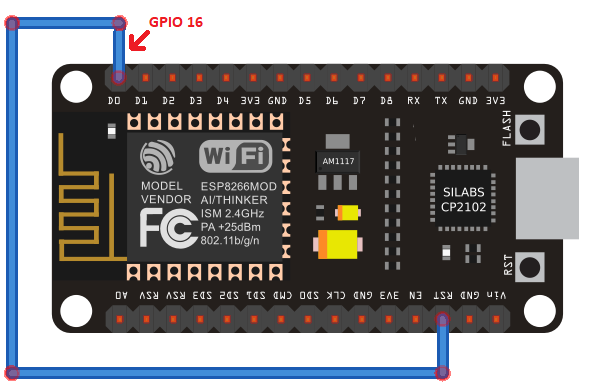
\includegraphics[width=\linewidth]{ESP8266_timed_deepsleep.png}
						    \caption{Sotwarově po daném čase}
						  \end{subfigure}
						  \begin{subfigure}[b]{0.4\linewidth}
						    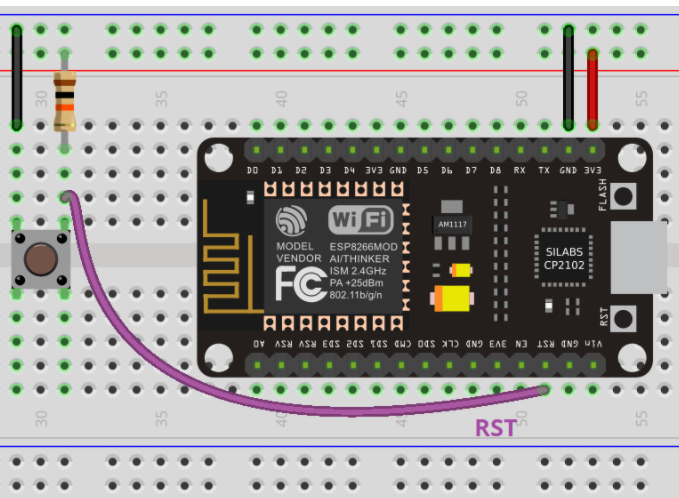
\includegraphics[width=\linewidth]{ESP8266_pressed_deepsleep.png}
						    \caption{Hardwarově}
						  \end{subfigure}
						  \caption{ESP8266 probuzení z deep sleep po daném čase}
						  \label{ESP8266_timed_pressed_deepsleep}
						\end{figure}


			\subsection{ESP32}
				ESP32 je starší model z řady ESP, který byl vydán v roce 2016. Tento mikročip má integrované WiFi i Bluetooth. Série ESP32 obsahuje mikroprocesor Tensilica Xtensa LX6 v dvou jádrové či jednojádrové verzi, který může operovat na 160 \si{MHz} nebo 240 \si{MHz}. SRAM je zde byla zvetšena na 520 \si{kB}. WiFi může dosáhnout rychlosti až 150 \si{Mbps} společně se zabezpečením WPA/WPA2. Kromě IPv4 je možnost použít i IPv6. ESP32 integruje 12 bitový analog-digitální převodník. Oproti ESP8266 je do tohoto modelu zabudován senzor teploty. ESP32 disponuje 36 GPIO piny. Další funkce jsou na obrázku \ref{ESP32_diagram}.

				\begin{figure}[h]
					\centering
					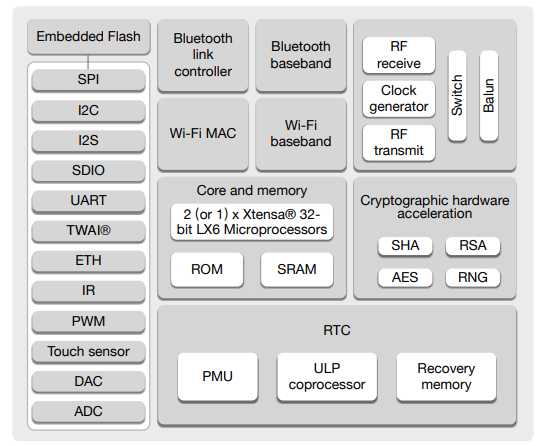
\includegraphics[width=14cm]{ESP32_diagram.png}
					\caption{ESP32 blokový diagram funkcí}
					\label{ESP32_diagram}
				\end{figure}



		\section{Komunikace mezi ESP a NETIO zásuvkou}

	\chapter{Metodika postupu}
		\section{Tvorba rozhraní}
		\section{Měření připojení k WiFi a odeslání HTTP requestu}
				Cílem měření je zjistění rychlostí a spotřeby připojení různými způsoby k přístupovému bodu a~následné porovnání případů. Do měření je také započítáné odesílání HTTP requestu zásuvce. Jsou vytvořeny celkem 4 případy akcí:
				\begin{itemize}
					\item {\bf statická IP adresa} - 	Zařízení dostane IP adresu, masku a bránu staticky staticky nakonfigurovanou. Na access pointu bude vyplé DHCP a komunikace nebyla zabezpečena.
					\item {\bf dynamická IP adresa} - Bude využit DHCP protokol, kde zařízení požádá DHCP server o IP adresu, kterou mu access point přidělí společně s bránou, maskou a~s~časem, kdy tato adresa platí. Při měření nebyl přístupový bod zabezpečen.
					\item {\bf Zabezpečené připojení} - Připojení na access point bude šifrované pomocí WPA2~-~PSK. DHCP server bude zapnut. Toto je simulace klasického uživatelského používání.
					\item {\bf Odeslání HTTP requestu} - Zařízení je připojené k WiFi. Odešle zprávu zásuvce a pokud dostane zpětnou vazbu od zásuvky, ukončí se činnost.
				\end{itemize}
				Ve všech scénářích bude měřeno zařízením {\bf ANALOG DISCOVERY 2} od Digilent. Frekvence procesoru je 160 \si{MHz} a AP je vzdálen 3,5 \si{m} od zásuvky a funkčního vzorku ovladače.
				\subsection{Spotřeba}
					Měřen bude úbytek napětí na bočníku\footnote{nízkoohmový rezistor} o velikosti určené u měření. V programu k měřícímu zařízení je možné stejně jako na osciloskopu vytvořit graf naměřených hodnot v dané vzorkovací frekvenci. Hodnoty napětí bude převedeno na hodnoty el. proudu pomocí Ohmova zákona $I = \frac{U}{R}$. Amplitudy el. proudu budou sečteny a vyděleny počtem vzorků {\bf[DOPLNIT VZOREC]}. Tato operace nám poskytne zjištění průměrného el. proudu ve scénáři. Spotřebu již vypočítáme dle:
					$$E = U \times \overline{I} \times \frac{t}{3600}$$
					Čas {\bf t} v sekundách je možné zjistit v následující kapitole.
				\subsection{Reakční čas}
					Z naměřeného případu bude vyjmuta klidová část a rozdíl mezi posledním a prvním vzorkem je poté reakční čas. V případě HTTP requestu nebude počítána část konfigurace WiFi. Společně s měřením byl na {\bf serial monitor} odesílány zprávy, kde se program nachází. Poté se vyjmula část, která dle serial monitoru nepatří do scénáře.

			\section{Ustálené stavy}
				Pro ustálené stavy byly navrhnuty jednoduché programy pro co nejlepší porovnání.
				\subsection{Spotřeba} \label{metodika:Ustálené stavy spotřeba}
					Cílem měření je nalézt stav s nejmenší spotřebou energie, jelikož finální prvek bude napájen z baterií je důležité co nejdelší výdrž. Pro měření bude použit {\bf ANALOG DISCOVERY} s jeho funkcí osciloskopu. Na napájení bude přidán bočník o velikosti 0,7 \si{\ohm}, 10,5 \si{\ohm} nebo 4,7 \si{\ohm} \footnote{Je nutné zvolit takový odpor, aby byl úbytek napětí měřitelný.}. Pomocí Ohmova zákona $ I = \frac{U}{R} $ je možné zjistit el. proud. Pro měření byly vybrány 3 scénáře.\\
					\begin{itemize}
						\item {\bf Kontinuální režim} - V tomto stanu není žádná funkce ESP vypnuta. Zařízení má nastavený určitý GPIO na tlačítko a monitoruje zda bylo zmáčknuto. ESP také má otevřenou sériovou komunikaci.
						\item {\bf Deep sleep} - ESP vypne vše až na RTC (kapitola viz. \ref{subsub:Deep sleep} na straně \pageref{subsub:Deep sleep}). Program zajišťuje probuzení ESP každých 5 \si{s} a odesílání zprávy na serial monitoring.
						\item {\bf Enable button} - ESP je vypnuto pomocí přivedené GROUND na pin ENABLE. Pro měření této situace není třeba specifický program
					\end{itemize}
					{\bf OBRÁZKY ZAPOJENÍ}
				\subsection{Probuzení z ustálených časů}
					Reakční doba byla změřena pomocí kamery. K tlačítku jsem připojil LED, místnost jsem izoloval od světla a zmáčknutí tlačítka a reakci zásuvky jsem natočil ve zpomaleném režimu s {\bf 240 snímky za sekundu}. Pro upravení videa jsem použil trial verzi programu {\bf Sony Vegas} (\viz{sonyvegaspostup}). Našel jsem rozsvícení LED tlačítka a rozsvícení LED zásuvky ve videu a ustřihl jsem tento úsek od zbytku videa. Program poskytuje zobrazení počtu snímku daného úseku. Reakční čas je následovně možný zjistit pomocí:
					$$ t = \frac{\textrm{Počet snímků úseku}}{\textrm{Počet snímků za sekundu}}$$
					\begin{figure}[h]
						\centering
						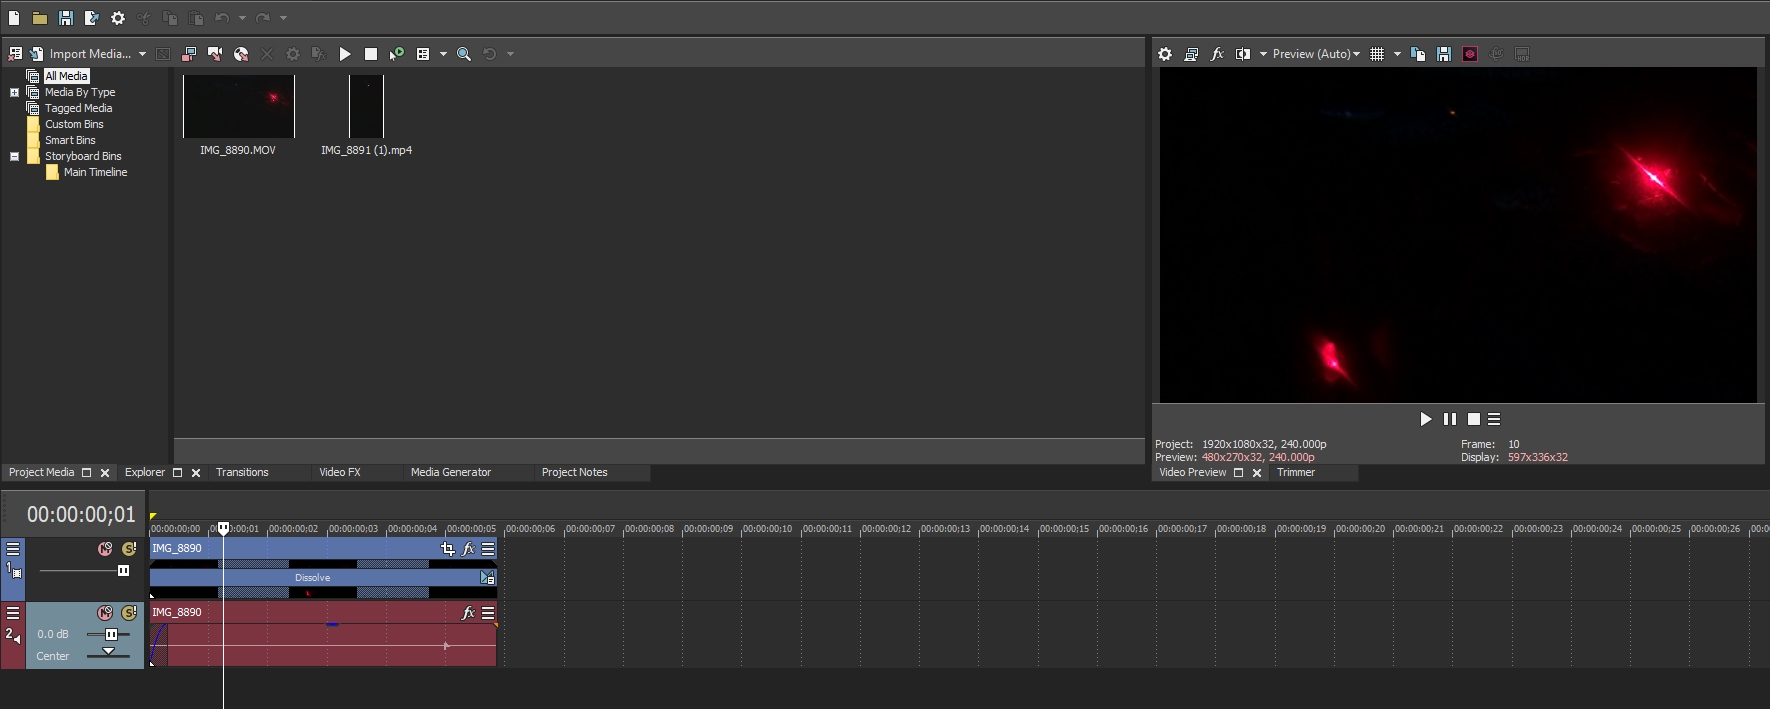
\includegraphics[width=12cm]{sonyvegaspostup.png}
						\caption{Ukázka postupu pro měření reakčních časů}
						\label{sonyvegaspostup}
					\end{figure}










	% 	Veškerý kód byl napsán v textovém editoru visual studio code s pluginem Platform.io, které usnadňuje některé metody používané v Arduino IDE.\\
	% 	Cílem webové stránky je umožnění připojení ovladače k uživatelské WiFi a následně vybrat pomocí IP adresy zařízení NETIO, které chceme ovládat. Stránka také musí umožňovat změnu reakce zásuvky na vyvolanou akci ovladačem.
	% 	\section{Nastavení webserveru}
	% 		Pro možnost nastavení ESP jsem vybral metodu konfigurace přes webserver jelikož po prvním spuštění ovladače ovladač není připojen k WiFi a úprava kódu není přívětivá možnost pro uživatele.

	% MĚŘENÍ
	\chapter{Měření spotřeby a času}
		\section{ESP8266}
			\subsection{Ustálené stavy}
				\subsubsection{Spotřeba}
					Spotřeba jednotlivých scénářů je měřena dle metodiky \ref{metodika:Ustálené stavy spotřeba} na straně \pageref{metodika:Ustálené stavy spotřeba}. Bočník pro měření úbytku napětí byl o velikosti 4,7 \si{\ohm}. \\

					\begin{figure}[h]
						\centering
						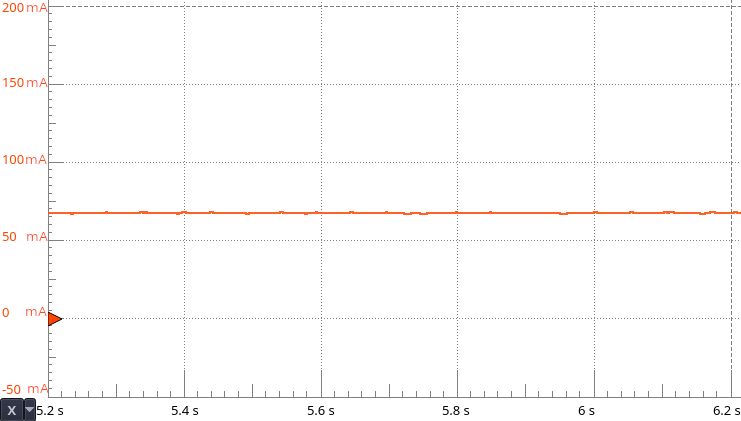
\includegraphics[width=13cm]{ESP8266_on_waiting.png}
						\caption{ESP8266 graf kontinuálního ustáleného stavu }
						\label{ESP8266_on_waiting}
					\end{figure}
					\begin{figure}[h]
						\centering
						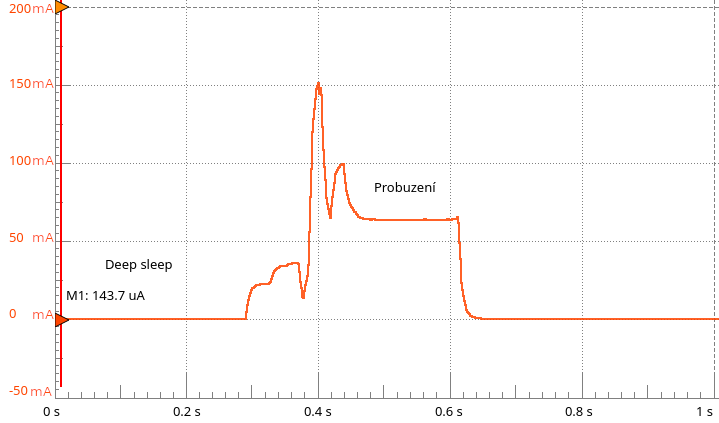
\includegraphics[width=13cm]{ESP8266_deepsleep_waiting.png}
						\caption{ESP8266 graf deep sleep ustáleného stavu}
						\label{ESP8266_on_waiting}
					\end{figure}

					Situace {\bf enable button} nebyla možná změřit zařízením {\bf ANALOG DISCOVERY 2} ani na bočníku o velikosti 0,7 \si{\ohm} kvůli velice nízkému úbytku napětí, který se v datasheetu WT8266 pohybuje v jednotkách \si{\micro A}. V tomto případě pro výpočty je použita hodnota, kterou určil výrobce v datasheetu.





			\subsection{Spotřeba ustálených stavů}
				Při měření spotřeby ustálených stavů bylo použito napájení z USB. Měřeno bylo zařízením \textbf{Analog Discovery 2} od společnosti \textbf{DIGILENT}. Tímto zařízením je měřeno napětí na rezistoru a dle Ohmova zákona: $I =\frac{U}{R}$ vypočítán eletrický proud. Napětí je 3,3 V.

				\subsubsection{ESP běží kontinuálně}
					Schéma zapojení \viz{ESP8266_on_schema} \\
					\obrazek{ESP8266_on_schema}{ESP8266 schéma zapojení kontinuálního ustáleného stavu}{10cm}{ESP8266_on_schema.png}
					Ústálený stav byl měřen za podmínek:
					\begin{itemize}
						\item Měřící rezistor má odpor 0,7 \si{\ohm}
						\item ESP8266 čeká na zmáčknutí tlačítka na pinu GPIO5
						\item ESP je neustále zapnuté, probíhá loop funkce pro kontrolu zmáčknutí
						\item Je připojeno k WiFi, je zaplý access point ESP, běží webserver
					\end{itemize}
		 			Při klidovém stavu byl naměřen eletrický proud průměrně 96,81 \si{mA} \viz{ESP8266_on_waiting}. Měření probíhalo 50 \si{s}. Pro jednotné porovnání je třeba vypočítat příkon:
						$$P = 96,81 \times 10^{-3}\si{A} \times 3,3 \si{ V}$$
		 			Dle rovnice se příkon rovná $ 319,5 \times 10^{-3}$ \si{\watt}\\
					\obrazek{ESP8266_on_waiting}{ESP8266 měření klidového stavu kontinualního režimu}{8cm}{ESP8266_on_waiting.png}

				\subsubsection{ESP vypnuté přes ENABLE pin}
					Schéma zapojení \viz{ESP8266_enable_schema}\\
					\obrazek{ESP8266_enable_schema}{ESP8266 schéma zapojení vypnutého ESP přes ENABLE pin}{10cm}{ESP8266_enable_schema.png}
					Měření proběhlo za podmínek:
					\begin{itemize}
						\item Měřící rezistor má odpor 10 \si{\ohm}
						\item pin enable byl připojen manuálně
					\end{itemize}
					Po připojení ESP8266 proud nevzrostl a drží se stále na 240 \si{\micro A}, což neodpovídá teoretickým hodnotám, které by se měly pohybovat okolo 3 \si{\micro A}
					\viz{1_enable}.\\
					\obrazek{1_enable}{Měření klidového režimu enable případu}{8cm}{1_enable.png}
					Pro výpočet bude jako průměrný odebraný proud použita hodnota uvedena v datasheetu což je 3 \si{\micro A}. Víme, že napětí je 3,3 \si{V} takže jsme schopni spočítat eletrický příkon:
				 		$$P = 3\times 10^{-6} \si{A}\times 3,3 \si{V}$$
					Výsledek je $9,9 \times 10^{-6}$ \si{\watt}.

				\subsubsection{Deep sleep režim}
					Schéma zapojení \viz{ESP8266_deepsleep_schema}\\
					\obrazek{ESP8266_deepsleep_schema}{ESP8266 schéma uvedené v deep sleep stavu}{10cm}{ESP8266_deepsleep_schema.png}
					Kvůli citlivosti Analog Discovery 2 nejsme schopni změřit spotřebu deep sleep režimu, je nutné změřit microampérmetrem. Pro výpočet spotřebované energie dosadíme za průměrný elektrický proud hodnotu z datasheetu, která odpovídá 20 \si{\micro A}. Spočítáme elektrický příkon:
						$$P = 20\times 10^{-6} \si{A}\times 3,3 \si{V}$$
					Ten v této situaci odpovídá hodnotě $66 \times 10^{-6}$ \si{\watt}.

				\subsubsection{Shrnutí výsledků měření spotřeby}
					Dle měření (\viztab{ESP8266 klidové režimy}) nejmenší spotřeba je pokud je ESP8266 vypnuté protože nepracuje žádná část ovladače, díky tomu ovladač je schopen vydržet na bateriích dlouhou dobu. Na druhé straně stojí kontinuální stav, kde ESP nevypne žádnou část a neustále běží. Kompromis je deep sleep, kdy ESP určité části aby ušetřil energii.

					\begin{table}[h]
						\centering
						\caption{ESP8266 porovnání ustálených stavů}
						\begin{tabular}{||l|r r||}
							\hline
							Ustálený stav & I($A$) & P($W$)\\
							\hline
							Kontinuální & $96,81 \times 10^{-3}$ & $319,5 \times 10^{-3}$\\
							Enable & $3,00\times 10^{-6}$ & $9,9 \times 10^{-6}$\\
							Deep sleep & $20,00\times 10^{-6}$ & $66,0 \times 10^{-6}$\\
							\hline
						\end{tabular}
						\label{ESP8266 klidové režimy}
					\end{table}

			\subsection{Reakční čas jednotlivých situací}

				\begin{table}[]
					\centering
					\caption{ESP8266 porovnání reakčního času jednotlivých situací}
					\begin{tabular}{||l|r||}
						\hline
						Ustálený stav & t(ms)\\
						\hline
						Kontinuální & {\bf 196}\\
						Enable & {\bf 3 208}\\
						Deep sleep & {\bf 983}\\
						\hline
					\end{tabular}
					\label{ESP8266 klidové režimy čas}
				\end{table}

				\subsubsection{Porovnání reakčních časů}
					Nejrychlejší reakce byla pokud ESP8266 bylo neustále zapnuto. Nejpomalejší naopak bylo pokud ESP8266 bylo nutné zapnout, je to z důvodu načtení sketche do operační paměti, načtení konfigurace WiFi a následnému připojení \viztab{ESP8266 klidové režimy čas}.






			% \subsection{Rychlost WiFi připojení}
			% 	Cílem měření je zjistění rychlostí připojení různými způsoby k přístupovému body, spotřeby a následné porovnání případů. Všechna měření byla provedena za podmínek:
			%
			% 	\begin{itemize}
			% 		\item Zařízení bylo napájeno z USB
			% 		\item Měřeno bylo pomocí úbytku napětí na rezistoru o velokosti 0,7 \si{\ohm}
			% 		\item Přístupový bod se nachází 3,5 \si{m} od zařízení
			% 	\end{itemize}
			%
			% 	\subsubsection{Dynamické přidělení IP adresy}
			% 		Měření proběhlo za použití DHCP protokolu, kdy zařízení požádá DHCP server o IP adresu, kterou mu Access point přidělí společně s bránou, maskou a s časem, kdy tato adresa platí. Při měření nebyl přístupový bod zabezpečen.\\
			% 		\obrazek{ESP8266_network_dynamic}{Měření dynamického připojení k AP}{8cm}{ESP8266_network_dynamic.png}
			% 		Měření bylo provedeno 5x. Průměrný čas se pohybuje okolo 4 652 \si{ms}. Jak je možno vidět na grafu (\viz{ESP8266_network_dynamic}), tak dvě WiFi připojení trvaly o 2 sekundy kratší dobu. ESP8266 se totiž zapíše do \textbf{DHCP client listu}, a má tak rezervovanou IP adresu, což znamená, že přiřazení proběhne rychleji.
			%
			% 	\subsubsection{Statické přidělení IP adresy}
			% 		Použita byla statická adresa, která byla přidělena ESP8266 před připojením na AP. Přístupový bod nebyl zabezpečen. DHCP server byl vypnut.
			% 		\obrazek{ESP8266_network_static}{Měření statického připojení k AP}{8cm}{ESP8266_network_static.png}
			% 		Měření proběhlo 5x. Průměrný čas byl 3238 \si{ms}.\\
			% 		\viz{ESP8266_network_static}
			%
			% 	\subsubsection{Zabezpečený AP}
			% 			Připojení na access point je šifrované pomocí WPA2-PSK. IP adresa je na ESP nastavena staticky. DHCP server je zapnut.
			% 			\obrazek{ESP8266_network_static_security}{Měření zabezpečeného připojení k AP}{8cm}{ESP8266_network_static_security.png}
			% 			Průměrný čas byl 4709 \si{ms}.\\
			% 			\viz{ESP8266_network_static_security}
			%
			% 	\subsubsection{Shrnutí výsledků rychlostí WiFi nastavení}
			% 		Z výsledků měření (\viztab{WiFi porovnání v sekundách}) je nejrychlejší připojení pomocí statické IP adresy, nicméně je velice náročné nastavit IP adresu, masku a bránu pro běžného uživatele. Připojení s DHCP je pomalejší průměrně o 1 \si{s} než případ se statickou IP adresou. DHCP vyniká jednoduchostí použití pro běžného uživatele. K zabezpečené WiFI trvá stejně dlouho jako s DHCP.
			%
			% 		\begin{table}[]
			% 			\centering
			% 			\caption{ESP8266 Porovnání reakční doby připojení k WiFi}
			% 			\begin{tabular}{||c|c c c||}
			% 				\hline
			% 				Pořadí & Dynamické & Statické & Zapezpečené\\
			% 				& (ms) & (ms) & (ms)\\
			% 				\hline
			%
			% 				1. & 5 300 & 3 143 & 4 606\\
			% 				2. & 5 300 & 3 143 & 4 606\\
			% 				3. & 3 619 & 3 143 & 4 606\\
			% 				4. & 5 300 & 3 143 & 4 606\\
			% 				5. & 3 627 & 3 143 & 4 606\\
			% 				\hline
			% 				{\bf Průměr} & {\bf 4 629} & {\bf 3 143} & {\bf 4 606}\\
			% 				\hline
			%
			% 			\end{tabular}
			% 			\label{WiFi porovnání v sekundách}
			% 		\end{table}
			%
			%
			% \subsection{Rychlost odeslání HTTP requestu}
			% 	Cílem měření je zjistit čas odesílání HTTP requestu a následné odpovězení zásuvky NETIO. Pokus byl proveden za podmínek:
			% 	\begin{itemize}
			% 		\item Napájeno z USB
			% 		\item Měřeno pomocí úbytku napětí na rezistoru o velitosti 0,7 \si{\ohm}
			% 		\item ESP8266 zkontroluje připojení k WiFi a pokud není navázáno, pokusí se ho navázat
			% 		\item Načtení uložené konfigurace WiFi z flash paměti trvá 300 \si{ms}
			% 		\item ESP ukončí reakci, pokud dostane zpětnou vazbu od zásuvky
			% 	\end{itemize}
			% 	\viz{ESP8266_http}
			% 	\obrazek{ESP8266_http}{ESP8266 měření odesílání HTTP requestu včetně reakce zásuvky}{8cm}{ESP8266_http.png}
			% 	Jelikož ESP přestane reagovat až po odpovězení zásuvky, dokážeme zjistit celkový čas včetně zapnutí, zkontrolování WiFi připojení, sestavení a odeslání HTTP requestu, reakce zásuvky a zpracování HTTP zprávy
			% 	\viztab{HTTP odeslání}.
			% 	\begin{table}[]
			% 		\centering
			% 		\caption{Čas odeslání HTTP requestu včetně reakce zásuvky}
			% 		\begin{tabular}{||c|c||}
			% 			\hline
			% 			Pořadí & HTTP request\\
			% 			& (ms)\\
			% 			\hline
			% 			\hline
			% 			1. & 732\\
			% 			2. & 645\\
			% 			3. & 732\\
			% 			4. & 732\\
			% 			5. & 747\\
			% 			\hline
			% 			{\bf Průměr} & {\bf 718}\\
			% 			\hline
			% 		\end{tabular}
			% 		\label{HTTP odesílání}
			% 	\end{table}

			\subsection{Spotřeba jednotlivých operací}
				Spotřebu budeme měřit pro jednotlivé situace WiFi a odesílání HTTP requestu. Pro tyto situace využijeme data z měření v kapitolách 4.1.3 a 4.1.4. Měření WiFi připojení probíhalo za vzorkovací frekvence 160 Hz a HTTP komunikace za 68,275 Hz. Z veličin, které známe, lze vypočítat \textbf{spotřebovanou energii}:
				$$E = P \times t$$
				$$E = U \times I \times t$$

				\begin{table}[h]
					\centering
					\caption{ESP8266 Spotřeba operací}
					\begin{tabular}{||l| r r r r |r||}
						\hline
						Operace & U(V) & I($mA$) & t($ms$) & P($mW$) & \textbf{E}($\mu Wh$)\\
						\hline
						\hline
					Dynamické připojení & 3,3 & 89,5 & 5 300 & 295 & \textbf{435}\\
					Statické připojení & 3,3 & 83,0 & 3 143 & 274 & \textbf{239}\\
					Zabezpečené připojení & 3,3 & 90,9 & 4 606 & 300 & \textbf{383}\\
					HTTP komunikace & 3,3 & 84,8 & 732 & 280 & \textbf{57}\\
					\hline
					\end{tabular}
					\label{Spotreba_operaci}
				\end{table}

				\subsubsection{Shrnutí výsledků spotřeby operací}
					Z tabulky \ref{Spotreba_operaci} je možné vidět, že {\bf příkon P} je téměř totožný v každé operaci. Největší rozdíl, který ovlivňuje spotřebu, je čas, za který se úkon vykoná. Jelikož {\bf připojení pomocí statické IP adresy} trvalo nejkratší dobu, má také nejmenší spotřebu.\\
					Samotná {\bf komunikace HTTP} má nejnižší spotřebu ze všech definovaných operací a jeden cyklus operace spotřebuje zanedbatelné množství energie.


		\section{ESP32}

			\subsection{Spotřeba ustálených stavů}

				\subsubsection{Kontinuální}

				\subsubsection{Enable}

				\subsubsection{Deep sleep}

			\subsection{Reakční čas jednotlivých situací}
				Získání reakčních časů jednotlivých možností zapojení ESP32 proběhlo stejným způsobem jako u ESP8266 (\viz{sonyvegaspostup} na straně \pageref{sonyvegaspostup}) tzn. Náhrál jsem reakci na kameru v 240 snímcích za sekundu, vystřihl jsem úsek, kde zásuvka reaguje, a převedl jsem snímky na čas.

				\begin{table}[h]
					\centering
					\caption{ESP32 porovnání reakčního času jednotlivých situací}
					\begin{tabular}{||l|r||}
						\hline
						Ustálený stav & t(ms) \\
						\hline
						Kontinuální & {\bf 188} \\
						Enable & {\bf 2 333} \\
						Deep sleep & {\bf 1 071} \\
						\hline
					\end{tabular}
					\label{ESP32 klidové režimy čas}
				\end{table}

		\section{Porovnání získaných výsledků}
			\subsection{Reakční časy stavů}
			Z tabulky \ref{Porovnání klidové režimy čas} je možné vidět jak si platformy vedly proti sobě. \\
			Pokud ovladač neustále běží s připojenou WiFi čas reakce je velmi rychlý a v obou případech uživatel nepostřehne prodlevu mezi aktivací ovladače a sepnutí relé v zásuvce. Časy mezi platformami se liší minimálně a rozdíl se pohybuje v rámci milisekund, přesto je ESP32 lehce rychlejší. \\
			Zapnutí vypnutého ESP, následné načtení a připojení k WiFi je nejdelší ze všech scénářů, který trvá několik sekund. Pro uživatele je velice pomalé a v realném produktu dle mého názoru zcela nepoužitelné. I přesto je ESP32 je mnohem rychlejší a to zhruba o 1 \si{s}. \\
			Deep sleep je alternativa mezi kontinuálním a vypnutým stavem. ESP totiž vypne vetšinu svých částí. Díky tomu je schopno relativně rychle zareagovat na budící signál. Reakce obou ovladačů je cirka 1 \si{s}. Zde vede ESP8266, které je zhruba o 100 \si{ms} pomalejší.

			\begin{table}[h]
				\centering
				\caption{Porovnání reakčních časů ústálených stavů platforem}
				\begin{tabular}{||l|r r||}
					\hline
					Ustálený stav & ESP8266 & ESP32 \\
					& (ms) & (ms) \\
					\hline
					Kontinuální & {\bf 196} & {\bf 188}\\
					Enable & {\bf 3 208} & {\bf 2 333}\\
					Deep sleep & {\bf 983} & {\bf 1 071}\\
					\hline
				\end{tabular}
				\label{Porovnání klidové režimy čas}
			\end{table}



% KONEC MĚŘENÍ


	\chapter{Vytvoření funkčních vzorků}
	\chapter{Závěr}

	\listoftables

	\listoffigures

	\prilohy{
		\kapitola{Příloha}
	}
	\literatura{
		\urll{ESP8266}{ESP8266}{Wireless-Tag Technology Co.,Limited}{Irvine (CA)}{Wireless-Tag}{2021}{\today}{https://www.tme.com/Document/12266bdd8a30eeb152305461b089a151/WT8266-S1.pdf}
		\wiki{DHCP protokol wiki}{DHCP protokol}{2021}{\today}{https://en.wikipedia.org/wiki\_Dynamic\_Host\_Configuration\_Protocol}
	}

\end{document}
